\documentclass{article}
\usepackage[utf8]{inputenc}
\usepackage[T1]{fontenc}
\usepackage{graphicx}
\usepackage{hyperref}
\usepackage{geometry}
\geometry{margin=1in}

\title{CABINET}
\date{Encyclopaedia Britannica (1771)}

\begin{document}
\maketitle

\section*{Historical source}
\textbf{Entry ID:} \texttt{entry-cabinet-2464} \\
\textbf{Volume ID:} 144133902 \\
\textbf{Character Count:} 762

\subsection*{Extracted Text}
CABINET, or CazBISY, the molt retired place in the finer part of a building, fet spart for writing, flu- dying, or preserving any thing that is precious.

A complete apartment conflicts of a hall, anti-cham- biz, chamber, and cobots, with a gallery on one files. Hence day, a number of paintings, curtains, ev. CAIBERT also denotes a piece of journer's workmanflap, being a kind of prels or cheft, with several doors and drawers.

There are common cabinets of oak or of chefnut, varnified cabbers of China and Japan, cabinets of in- leaf work, and fone of ebony, or the like force and precious woods.

Formerly the Dutch and German cabinets were much allemented in France, but are now quite out of fibre, as well as the cabinets of ebony, which came from Venice.



\section*{Source record}
\begin{itemize}
\item \textbf{Dataset:} \texttt{NationalLibraryOfScotland/encyclopaedia\_britannica\_illustrated}
\item \textbf{Dataset Revision:} \texttt{309f765b1ecc83e0a7f7762e44b4a927a7555443}
\item \textbf{Page ID:} \texttt{britannica:309f765b1ecc83e0a7f7762e44b4a927a7555443:train:2464} \\
  \textbf{Filename:} \texttt{page-2464-24f450326eee.jpg} \\
  \textbf{Row Index:} 2464 \\
  \textbf{SHA256:} \texttt{24f450326eee13b0...}
\end{itemize}

\begin{figure}[h]
\centering
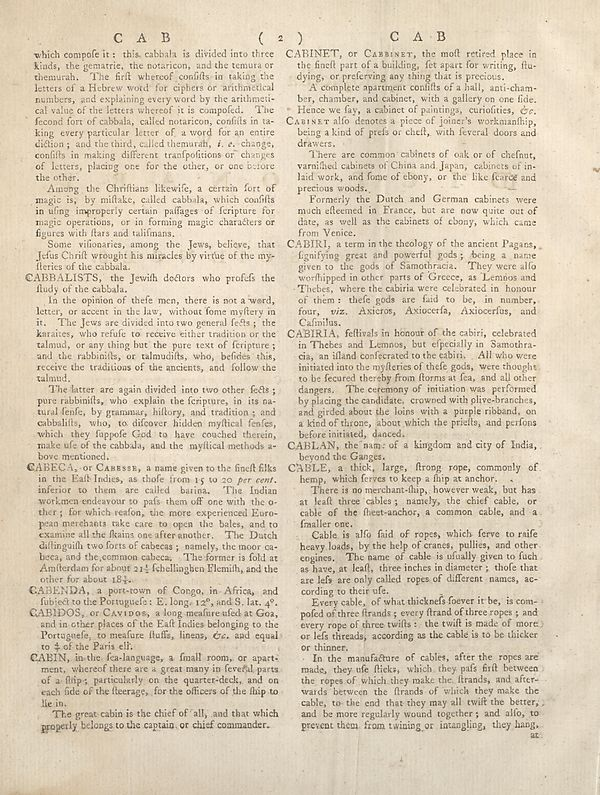
\includegraphics[width=0.85\textwidth]{../scans/page-2464-24f450326eee.jpg}
\caption*{Source scan: \texttt{page-2464-24f450326eee.jpg}}
\end{figure}

\end{document}
